% Options for packages loaded elsewhere
\PassOptionsToPackage{unicode}{hyperref}
\PassOptionsToPackage{hyphens}{url}
\PassOptionsToPackage{dvipsnames,svgnames,x11names}{xcolor}
%
\documentclass[
  letterpaper,
  DIV=11,
  numbers=noendperiod]{scrreprt}

\usepackage{amsmath,amssymb}
\usepackage{lmodern}
\usepackage{iftex}
\ifPDFTeX
  \usepackage[T1]{fontenc}
  \usepackage[utf8]{inputenc}
  \usepackage{textcomp} % provide euro and other symbols
\else % if luatex or xetex
  \usepackage{unicode-math}
  \defaultfontfeatures{Scale=MatchLowercase}
  \defaultfontfeatures[\rmfamily]{Ligatures=TeX,Scale=1}
\fi
% Use upquote if available, for straight quotes in verbatim environments
\IfFileExists{upquote.sty}{\usepackage{upquote}}{}
\IfFileExists{microtype.sty}{% use microtype if available
  \usepackage[]{microtype}
  \UseMicrotypeSet[protrusion]{basicmath} % disable protrusion for tt fonts
}{}
\makeatletter
\@ifundefined{KOMAClassName}{% if non-KOMA class
  \IfFileExists{parskip.sty}{%
    \usepackage{parskip}
  }{% else
    \setlength{\parindent}{0pt}
    \setlength{\parskip}{6pt plus 2pt minus 1pt}}
}{% if KOMA class
  \KOMAoptions{parskip=half}}
\makeatother
\usepackage{xcolor}
\setlength{\emergencystretch}{3em} % prevent overfull lines
\setcounter{secnumdepth}{5}
% Make \paragraph and \subparagraph free-standing
\ifx\paragraph\undefined\else
  \let\oldparagraph\paragraph
  \renewcommand{\paragraph}[1]{\oldparagraph{#1}\mbox{}}
\fi
\ifx\subparagraph\undefined\else
  \let\oldsubparagraph\subparagraph
  \renewcommand{\subparagraph}[1]{\oldsubparagraph{#1}\mbox{}}
\fi


\providecommand{\tightlist}{%
  \setlength{\itemsep}{0pt}\setlength{\parskip}{0pt}}\usepackage{longtable,booktabs,array}
\usepackage{calc} % for calculating minipage widths
% Correct order of tables after \paragraph or \subparagraph
\usepackage{etoolbox}
\makeatletter
\patchcmd\longtable{\par}{\if@noskipsec\mbox{}\fi\par}{}{}
\makeatother
% Allow footnotes in longtable head/foot
\IfFileExists{footnotehyper.sty}{\usepackage{footnotehyper}}{\usepackage{footnote}}
\makesavenoteenv{longtable}
\usepackage{graphicx}
\makeatletter
\def\maxwidth{\ifdim\Gin@nat@width>\linewidth\linewidth\else\Gin@nat@width\fi}
\def\maxheight{\ifdim\Gin@nat@height>\textheight\textheight\else\Gin@nat@height\fi}
\makeatother
% Scale images if necessary, so that they will not overflow the page
% margins by default, and it is still possible to overwrite the defaults
% using explicit options in \includegraphics[width, height, ...]{}
\setkeys{Gin}{width=\maxwidth,height=\maxheight,keepaspectratio}
% Set default figure placement to htbp
\makeatletter
\def\fps@figure{htbp}
\makeatother

\KOMAoption{captions}{tableheading}
\makeatletter
\makeatother
\makeatletter
\@ifpackageloaded{bookmark}{}{\usepackage{bookmark}}
\makeatother
\makeatletter
\@ifpackageloaded{caption}{}{\usepackage{caption}}
\AtBeginDocument{%
\ifdefined\contentsname
  \renewcommand*\contentsname{Table of contents}
\else
  \newcommand\contentsname{Table of contents}
\fi
\ifdefined\listfigurename
  \renewcommand*\listfigurename{List of Figures}
\else
  \newcommand\listfigurename{List of Figures}
\fi
\ifdefined\listtablename
  \renewcommand*\listtablename{List of Tables}
\else
  \newcommand\listtablename{List of Tables}
\fi
\ifdefined\figurename
  \renewcommand*\figurename{Figure}
\else
  \newcommand\figurename{Figure}
\fi
\ifdefined\tablename
  \renewcommand*\tablename{Table}
\else
  \newcommand\tablename{Table}
\fi
}
\@ifpackageloaded{float}{}{\usepackage{float}}
\floatstyle{ruled}
\@ifundefined{c@chapter}{\newfloat{codelisting}{h}{lop}}{\newfloat{codelisting}{h}{lop}[chapter]}
\floatname{codelisting}{Listing}
\newcommand*\listoflistings{\listof{codelisting}{List of Listings}}
\makeatother
\makeatletter
\@ifpackageloaded{caption}{}{\usepackage{caption}}
\@ifpackageloaded{subcaption}{}{\usepackage{subcaption}}
\makeatother
\makeatletter
\@ifpackageloaded{tcolorbox}{}{\usepackage[many]{tcolorbox}}
\makeatother
\makeatletter
\@ifundefined{shadecolor}{\definecolor{shadecolor}{rgb}{.97, .97, .97}}
\makeatother
\makeatletter
\makeatother
\ifLuaTeX
  \usepackage{selnolig}  % disable illegal ligatures
\fi
\IfFileExists{bookmark.sty}{\usepackage{bookmark}}{\usepackage{hyperref}}
\IfFileExists{xurl.sty}{\usepackage{xurl}}{} % add URL line breaks if available
\urlstyle{same} % disable monospaced font for URLs
\hypersetup{
  pdftitle={Canseza Avağ Erdurak},
  colorlinks=true,
  linkcolor={blue},
  filecolor={Maroon},
  citecolor={Blue},
  urlcolor={Blue},
  pdfcreator={LaTeX via pandoc}}

\title{Canseza Avağ Erdurak}
\author{}
\date{}

\begin{document}
\maketitle
\ifdefined\Shaded\renewenvironment{Shaded}{\begin{tcolorbox}[borderline west={3pt}{0pt}{shadecolor}, boxrule=0pt, interior hidden, enhanced, breakable, frame hidden, sharp corners]}{\end{tcolorbox}}\fi

\renewcommand*\contentsname{Table of contents}
{
\hypersetup{linkcolor=}
\setcounter{tocdepth}{2}
\tableofcontents
}
\bookmarksetup{startatroot}

\hypertarget{introduction}{%
\chapter*{Introduction}\label{introduction}}
\addcontentsline{toc}{chapter}{Introduction}

This progress journal covers Canseza Avağ Erdurak's work during their
term at \href{https://mef-bda503.github.io/fall22/}{BDA 503 Fall 2022}.

Each section is an assignment or an individual work.

\bookmarksetup{startatroot}

\hypertarget{bda503-assignment1}{%
\chapter{BDA503-Assignment1}\label{bda503-assignment1}}

Canseza Avağ Erdurak\\
today

\hfill\break

I am Canseza Avağ Erdurak. I graduated from Management Information
Systems, Boğaziçi University in 2011. Since then, I always dreamed about
having a master's degree. Being a MEFIAN made my dream come through. I
am super excited to be a part of this programme. I was less interested
in coding staff when I was an undergradute. I'm ended up like coding is
not that boring after I started to work as a BI Developer. Being a BI
Developer restricted me in a way that I could not involve in building a
structure of the reports I am working on. I decided to choose a path
that I could get my hands dirty in both BI and DWH jobs. I work as a BI
Engineer in Pegasus Airlines since July 2018. It started to feel like I
should step in the field of AI to make my job better and to be more
satisfied at work. As a BI Engineer, I only provide data and support for
architectural structure in AI Projects. However, I want to initiate and
lead AI projects on my own. I believe that I am passionate,
intellectually capable, and prepared to set out on this exhilarating and
challenging path. I look forward to learn exploratory data analysis,
machine learning and automation in R.

Here is the link of my linkedin profile :
\url{https://www.linkedin.com/in/cansezaavag/}.

\hypertarget{rstudio-global-2022-conference-talks-save-an-ocean-of-time}{%
\section{RStudio Global 2022 Conference Talks : Save an Ocean of
Time}\label{rstudio-global-2022-conference-talks-save-an-ocean-of-time}}

The speaker, \textbf{Danielle Dempsey} works for CMAR that has over 250
oceanographic sensors deployed around the coast of Nova Scotia, Canada.
Together, these generate around 4 million rows of data every year. Her
challenge was to compile all of data stored in Excel files in different
formats into a nice, tidy format that they could post online for any
interested stakeholder to download and use in their own analysis.

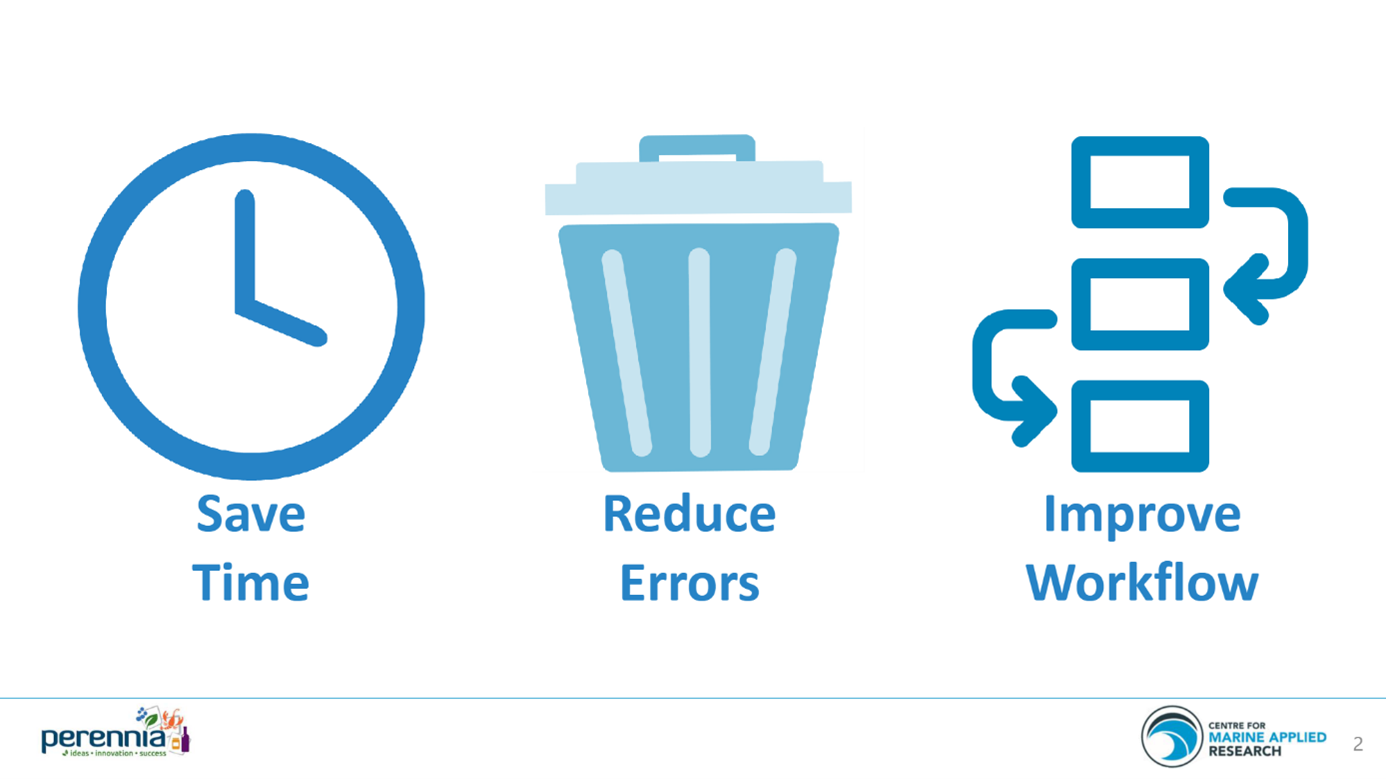
\includegraphics{./writingcode.png}

She mentions about how skeptical her manager was at first, since there's
an existing process that's already ``good enough''. However, she was
decided not to proceed old-fashioned methods like copy+paste. She was
not confident in data wrangling and package development skills. She
spent time in coding to save time. She used Tidyverse packages mostly in
her project. It took 9 months rather than 2 years to complete the task.
If she didn't change the way how the work is done, she couln't get the
results below. Skills that you learn working on one coding project are
often transferable to other projects. She has used packages and skills
she developed for further projects. She says how easier it is to train
new people getting them on board. Errors can pop up anywhere in data
since humans are involved. Writing code makes to find and reduce errors
in your dataset. It makes get clients more confident in data and make
analysis with that data more reliable. Automate your data wrangling make
your workflow more traceable and reproducible especially compared to
copying and pasting. At the end, she mentions about how her manager
changed her mind over streamlining a workflow. Her manager made him a
hand-made present shaped as Super ``R'' so that she thought ``R can do
anything that we put our minds to.'' It think this metaphor she puts
made me chose Danielle's talk for the assignment : ``Making a salad left
in the fridge. Most of the time, it tastes ok but eventually you will
get something that doesn't taste quite right. Because you have no record
of what went into that salad it's really hard to tell what exactly is
making it taste funny, and it's also hard to avoid making the same
mistake in the future. You can't take the dressing back out of the
salad. In contrast, writing code is like writing and following a recipe.
You can follow it step by step to get a delicious salad every time. As a
bonus, you can give that recipe to a friend so they can make their own
salad or help you make dinner.'' This conference talk made me impressed
and motivated about my philosophy at work. At first, I go over process
of how clients complete an existing job. Then, I start writing SQL codes
to automate workflow. When clients are totally on board with me, they
bring on new projects more reluctantly to work for. It has also changed
the way how they make use of DWH/BI skills on processes and help them
make more informative decisions about work.

\textbf{Video link :}
\url{https://www.rstudio.com/conference/2022/talks/save-ocean-of-time-streamline/}

\textbf{Talk materials' link :}
\url{https://github.com/dempsey-CMAR/2022_rstudio_conf}

\hypertarget{r-posts-relevant-to-my-interests}{%
\section{3 R Posts Relevant to My
Interests}\label{r-posts-relevant-to-my-interests}}

\hypertarget{tidyverse}{%
\subsection{Tidyverse}\label{tidyverse}}

When I started to watch conference talk that I mentioned above, I
realized I could do anything related to data wrangling I did so far in
Pegasus by using R. So, I decided to elaborate on this article.
Tidyverse has 8 core packages named \textbf{ggplot2, dplyr, tidyr,
readr, purrr, tibble, stringr} and \textbf{forcats}.

\begin{enumerate}
\def\labelenumi{\arabic{enumi}.}
\tightlist
\item
  \textbf{Data Visualization and Exploration}
\end{enumerate}

\begin{itemize}
\tightlist
\item
  \textbf{ggplot2} is used to create data visualizations like bar
  charts, pie charts, histograms, scatterplots, error charts, etc.
\end{itemize}

\begin{enumerate}
\def\labelenumi{\arabic{enumi}.}
\setcounter{enumi}{1}
\tightlist
\item
  \textbf{Data Wrangling and Transformation}
\end{enumerate}

\begin{itemize}
\item
  \textbf{Dplyr} is known for data manipulation. It has five important
  functions namely mutate(), select(), filter(), summarise() and
  arrange(). These functions are used with group\_by().
\item
  \textbf{Tidyr} helps create clean data.
\item
  \textbf{Stringr} has many functions for data cleaning and data
  preparation. All functions in this library starts with ``str'' and
  take a string vector as a first argument.
\item
  \textbf{Forcats} handles issues like changes the orders of values in
  vectors, reordering the vectors, etc.
\end{itemize}

\begin{enumerate}
\def\labelenumi{\arabic{enumi}.}
\setcounter{enumi}{2}
\tightlist
\item
  \textbf{Data Import and Management}
\end{enumerate}

\begin{itemize}
\item
  \textbf{Readr} helps read rectangular data such as that with file
  formats tsv, csv, delim, fwf, etc. in a simple and speedy way.
\item
  \textbf{Tibble} is a form of a data.frame which includes the useful
  parts of it and discards the parts that are not so important.
\end{itemize}

\begin{enumerate}
\def\labelenumi{\arabic{enumi}.}
\setcounter{enumi}{3}
\tightlist
\item
  \textbf{Functional Programming}
\end{enumerate}

\begin{itemize}
\tightlist
\item
  \textbf{Purrr} turns messed-up codes into simpler ones.
\end{itemize}

\textbf{Article :}
\url{https://www.geeksforgeeks.org/what-are-the-tidyverse-packages-in-r-language/}

\hypertarget{uncover-the-r-applications}{%
\subsection{Uncover the R
Applications}\label{uncover-the-r-applications}}

I watched many conference talks so that I could chose one for this
assignment. These talks make me wonder why R Programming Language is
used by top companies from various industries like banking, e-commerce,
finance, etc.

\textbf{Applications of R Programming :}

\begin{itemize}
\item
  \textbf{Finance :} R helps financial institutions perform downside
  risk measurement, adjust risk performance and utilize visualizations
  like candlestick charts, density plots, drawdown plots, etc.
  Time-series statistical processes of R are used to model the movement
  of financial industries' stock-market and predict the prices of
  shares. R provides financial data mining capabilities through its
  packages like quantmod, pdfetch, TFX, pwt, etc. Rshiny helps extract
  data from online assets.
\item
  \textbf{Banking :} R is most widely used for credit risk modeling and
  other forms of risk analytics.
  \href{https://data-flair.training/blogs/hadoop-tutorials-home/}{\emph{Hadoop}}
  is an ally of R in the fields like analysis of customer quality,
  customer segmentation, and retention.
\item
  \textbf{Healthcare :} R helps perform pre-clinical trials and analyze
  the drug-safety data. R is also used for statistical modeling in the
  field of epidemiology, where data scientists analyze and predict the
  spread of diseases.
\item
  \textbf{Social Media :} Some of the important statistical tools like
  sentiment analysis and other forms of social media data mining are
  used with R. Social media is used for potential customer segmentation
  and targeting them as new customers.
\item
  \textbf{E-commerce :} E-commerce companies use R is for analyzing
  cross-selling products to their customers. Various statistical
  procedures like linear modeling are necessary to analyze the purchases
  made by the customers as well as in predicting product sales.
  Furthermore, companies use R for carrying out A/B testing analysis
  across the pages of their products.
\item
  \textbf{Manufacturing :} Analyzing customer sentiment helps them
  optimize their product according to trending consumer interests and
  also to match their production volume to varying market demand. They
  also use R to minimize their production costs and maximize profits.
\end{itemize}

\textbf{Article :}
\url{https://data-flair.training/blogs/r-applications/}

\hypertarget{data-analysis}{%
\subsection{Data Analysis}\label{data-analysis}}

Analyzing data is key for success. I reviewed this article so that I
could have a sense of how data is analyzed through R. The project is
done to find out that how informative ingredients are for determining
price of skincare products. Hypothesis is brand will be much more
informative than ingredients to predict the price of a product. It's an
end-to-end analysis project from data analysis to machine learning
algorithm validation. The researcher mentions about experimental
limitations of the project. It is concluded the higher prices in
skincare products does not mean higher quality skincare ingredients. You
can go over details of analysis in the link below.

\textbf{Article :}
\url{https://towardsdatascience.com/data-analysis-ingredients-of-skincare-products-not-found-to-affect-product-price-c3593d123a4d}



\end{document}
